\chapter{Stromal and Oncogenic Regulation of Colonic Stem Cell Polarisation}
\label{04seq}

\section{Introduction}

% The cell communication information gathered this way can then be summarised as signalling pathways that define and connect the different populations of cells. Furthermore, the study of this interactome would aid towards understanding the interplay between the CRC organoid model and its TME. This can be achieved by comparing the cell communication results with the intracellular PTM signalling described in Qin et al. 2020 and seeing how cellular communications change in cultures mimicking an oncogenic setting.

As presented in Chapter \ref{01intro}, the colonic epithelium is a highly heterogeneous system with multiple specialised cell types. Supported by the \emph{Lgr5}\textsuperscript{+} colonic stem cells (CSCs) of the crypt, its homeostatic regulation relies on intrinsic and extrinsic cues, the latter of which predominately come from the stromal compartment. In the context of colorectal cancer (CRC), and under the classical progression model \cite{fearon_genetic_1990}, oncogenic mutations targeting \textit{Apc}, \textit{Kras}, \textit{Braf}, \textit{Smad4}, and/or \textit{Trp53} constitute intrinsic cues that are sufficient to induce a highly proliferative crypt-progenitor phenotype, the \acrfull{procsc} \cite{van_de_wetering_-catenintcf-4_2002}.
Therefore, in both the healthy colon and CRC a compartment of epithelial cells is maintained in a stem-like state, although by different mechanisms. 

This shared crypt-progenitor phenotype actually represents a broader compartment encompassing more than the canonical LGR5\textsuperscript{+} CSCs; with recent studies describing the existence of the \emph{Clu}\textsuperscript{+} revival stem cell state (revCSC). Reminiscent of foetal-like states, \acrshort{revcsc} p has been described as a small and non-hyperproliferative compartment involved in tissue regeneration after injury and suggested as a drug-tolerant persister state in CRC. 

However, the mechanisms of regulation between the different stem cell states largely remain unclear.
Involvement of cell extrinsic cues in the form of stroma-secreted ligands, coupled with the association of the TME with CRC progression, suggest that they must also pay a role in regulating the colonic epithelia. The cell extrinsic cues involve signalling pathways that overlap with those affected by the oncogenic mutations \colorbox{yellow}{Reference here\cite{sphyris_subversion_2021}, also spell out pathways?}, indicating a competition between intrinsic and extrinsic cues to regulate epithelial polarisation might take place during oncogenesis.

% Canonically, both stromal WNT/R-Spondin-1 ligands and APC-loss hyper-activate \textbeta-catenin signalling, whereas EGF and KRAS/BRAF mutations stimulate the MAPK pathway \cite{sphyris_subversion_2021}.

Thus, single-cell omic technologies are perfectly placed to understand polarisation of the epithelial compartment at a broader level and reveal the regulation of cell fates by competing cues.

In this Chapter I will explore via scRNA-seq how cell extrinsic and intrinsic cues co-regulate colonic epithelial fate using a heterocellular organoid culture system with both environmental and oncogenic perturbations. I will first characterise the different populations found in the heterocellular cultures, identify the different epithelial cell states and their compositional changes in response to intrinsic and extrinsic cues. Cellular dynamics approaches will reveal our understanding of the balance regulating the proCSC and revCSC states, and cell-cell communication analysis will suggest putative mechanisms of regulation. Finally, the findings will be contextualised with the broader literature leveraging published gene signatures.

The work presented here is part of Qin \& Cardoso Rodriguez et al. 2023 \cite{cardoso_rodriguez_single-cell_2023}, where it is shown accompanied with mass cytometry analyses carried out by Dr. Xiao Qin and whose results validate the scRNA-seq findings and shed light on the mechanisms of epithelia stem cell polarisation in this shared landscape.

\begin{figure}
    \centering
    \includegraphics{04seq/figs/4SEQ_ExpDesign.png}
    \caption{\textbf{A)} Multivariate scRNA-seq experimental design. WENR ligands were removed from all experimental conditions except for the niche factor control to ensure cell-cell signalling was not dominated by exogenous recombinant proteins (see Methods). \textbf{B)} Single-cell PHATE embedding illustrating epithelial cells, fibroblasts, and macrophages. \textbf{C)} PCAs of epithelial, fibroblast, and macrophage transcriptomes regulated by by organoid genotype and microenvironment. WENR, WNT3A, EGF, Noggin, and R-Spondin-1.}
    \label{fig:4exp}
\end{figure}

To directly compare how CRC oncogenic mutations and stromal cells regulate colonic epithelial differentiation, I performed a multivariate scRNA-seq analysis of wild-type (WT), \textit{shApc} (A), \textit{shApc} and \textit{Kras\textsuperscript{G12D/+}} (AK), and \textit{shApc}, \textit{Kras\textsuperscript{G12D/+}} and \textit{Trp53\textsuperscript{R172H/–}} (AKP) colonic organoids, in monoculture or co-cultured with colonic fibroblasts and/or macrophages (Figure \ref{fig:4exp}A). Fibroblasts are established regulators of intestinal epithelia \cite{roulis_fibroblasts_2016} and macrophages are the most profuse leukocytes in the colon \cite{isidro_colonic_2016}. A condition with WT organoids cultured with exogenous WNT3A, EGF, Noggin, and R-Spondin-1 (WENR) (commonly used to grow colonic organoids) was included as a defined mesenchymal niche factor control. 

Following data acquisition and initial preprocessing steps (see Chapter \ref{02methods}), epithelial cells, fibroblasts, and macrophages were jointly embedded in an integrated space and visualised by PHATE (Potential of Heat-diffusion for Affinity-based Trajectory Embedding) \cite{moon_visualizing_2019}. This embedding resolves the three distinct cell types as shown by expression of levels of canonical cell type markers (Figure \ref{fig:4exp}B). 
Cell-type-specific transcriptional changes were referenced against relevant control monoculture conditions (WT organoids for the epithelial cells) using the EMD score (see \ref{02methods}, and then summarised using PCA (Figure \ref{fig:4exp}C). Epithelial transcriptomes are differentially regulated by both CRC mutations (PC1, 26\%) and microenvironmental cues (PC2, 22\%), with A, AK, and AKP mutations progressively dysregulating their transcriptomic profiles. However, we found fibroblasts can only regulate WT and A epithelial cells (Figure \ref{fig:4exp}C). Although WENR ligands are thought to mimic a healthy stromal niche \cite{mahe_establishment_2013}, WT organoids + WENR ligands transcriptionally align with AK mutant organoids (not WT+fibroblasts as might be expected), indicating this widely used colonic organoid culture media induces a partial CRC-like transcriptome in WT epithelia (Figure \ref{fig:4exp}C).
Colonic fibroblast cells resolved into CD34\textsuperscript{hi} and CD34\textsuperscript{lo} subpopulations mimicking \textit{in vivo} stromal heterogeneity \cite{karpus_colonic_2019} (Figure \ref{sfig:defib}). CD34\textsuperscript{hi} and CD34\textsuperscript{lo} fibroblasts did not differentially regulate colonic epithelia (Figure \ref{sfig:deepibyfib}) and were subsequently treated as a heterogenous mesenchymal population. Bone marrow macrophages on the other hand presented as a continuum of cells aligned along and axis of inversely correlated expression of complement genes (like \emph{C1q}) and \emph{Hmox1}, see \ref{fig:4exp}), possibly indicating inflammation-related roles to be a major driver of heterogeneity within the macrophage cells \cite{naito_heme_2014}. However, we found that fibroblast and macrophage transcriptomes and compositional make-up were only regulated by co-culture with heterotypic cells but not altered by epithelial genotypes (Figures \ref{sfig:defib}, \ref{sfig:demac}). 


\section{Organoids recapitulate colonic epithelial cell states}

\begin{figure}[H]
    \centering
    \includegraphics{04seq/figs/4SEQ_INTctrl.png}
    \caption{\textbf{D)} PHATE embedding of 29,452 epithelial cells from the 17 organoid conditions coloured by cell-type clusters. CSC, colonic stem cell. proCSC, hyper-proliferative CSC. revCSC, revival CSC. DCS, deep crypt secretory cell. TA, Transit amplifying cell. \textbf{B)} Single-cell PHATE embeddings of epithelial cells from WT, WT+Fibroblasts, WT+WENR, and AK organoids coloured by cluster and overlaid with single-cell density.}
    \label{fig:4intepi}
\end{figure}

Epithelial cells from all conditions were integrated by reciprocal PCA (RPCA) \cite{hao_integrated_2021}, projected onto a shared PHATE embedding, and clustered into multiple cell-fates, including stem populations, transit amplifying (TA) cells, cells under ER stress, goblet and deep crypt secretory (DCS) cells, and early or late enterocytes (Figure \ref{fig:4intepi}A). 

While this integrated space presents a continuum of cells, density plots of 4 extremes in our experimental design matrix point towards some degree of polarisation (Figure \ref{fig:4intepi} B). The WT monoculture control spans a broad range in the embedding space and shows high density in the CSC to Enterocyte and Goblet/DCS differentiation axes. The WT cocultured with macrophages appears to show the highest density of cells around the revCSC state, whereas the AK monoculture is densest around the proCSC. Finally, the condition with exogenous WENR ligands seems to polarise both towards proCSC and revCSC..

The multiple epithelial compartments where identified and associated with the relevant clusters based on their expression of canonical markers of selected colon cell epithelia cell types (see Sup. Table \ref{tab:epimarkers} for more epithelial marker genes). Expression of these genes on the WT monoculture control reveals how the system recapitulates the basal (stem and TA), secretory, and absorptive compartments (Figure \ref{fig:4intepi} B). The stem compartment appears distributed along several clusters (proCSC, CSC, revCSC) and extends towards the TA cells. A state characterised by a clear ER stress response gene expression signature lays adjacent to the stem and TA compartments (Figure \ref{fig:4intepi} B).


\section{Oncogenic mutations and fibroblasts polarise epithelia towards distinct stem cell fates}

Compositional analysis via \acrfull{da} testing \cite{dann_differential_2022} is used to identify and quantify effects of perturbations on a system (see Chapter \ref{02methods} for more details). \acrshort{da} was thus used to determine the changes induced by stromal and oncogenic cues compared to the WT mono-culture organoid baseline, revealing that fibroblasts and CRC mutations have markedly different effects on epithelial cell-fate determination (Figure \ref{fig:4da}). 

\begin{figure}
    \centering
    \includegraphics{04seq/figs/4SEQ_DA.png}
    \caption{\textbf{F)} Epithelial PHATE overlaid with differentially abundant (DA) neighbourhoods in WT organoid + fibroblast co-cultures compared with WT organoid monocultures. \textbf{G)} Epithelial PHATE overlaid with DA neighbourhoods in AK/AKP organoid monocultures compared with WT organoid monocultures. \textbf{H)} Dot plot of epithelial clusters across organoid cultures coloured by log fold-change (Log FC) in neighbourhood abundance and sized by the number of neighbourhoods detected.}
    \label{fig:4da}
\end{figure}
\begin{figure}
    \centering
    \includegraphics{04seq/figs/4SEQ_DE.png}
    \caption{\textbf{I)} Gene expression signatures of epithelial clusters.}
    \label{fig:4de}
\end{figure}

Fibroblasts enrich for the revCSC population characterised by high expression of epithelial progenitor genes \textit{Clu}, \textit{Sox9}, \textit{Cd44}, and \textit{Cldn4} (Figures \ref{fig:4da}A, \ref{fig:4de}). In contrast, A, AK, and AKP mutations progressively polarise epithelia towards a hyper-proliferative proCSC state (Figure \ref{fig:4da} B). proCSCs express \textit{EphB2}, \textit{Birc5} (\textit{Survivin}), \textit{Lrig1}, \textit{Hmgb2}, and \textit{Rrm2} and are highly mitotic (\textit{Stmn1\textsuperscript{+}}, \textit{Mki67\textsuperscript{+}}, and \textit{Ccnb1\textsuperscript{+}}) (Figure \ref{fig:4de}). 

Both revCSC and proCSC are present in WT organoids at low levels alongside traditional \textit{Lgr5\textsuperscript{+}} CSCs, and these cells were found to also be enriched by A, AK, and AKP genotypes, but to a lesser extent than proCSC (\ref{fig:4da}C).

While the \acrshort{da} method employed essentially works at a pairwise level, I aggregated results from multiple comparisons across the experimental matrix (Figure \ref{fig:4da}C) to show how how fibroblasts can only induce revCSC in WT and \textit{shApc} epithelia, but not when cells contain both \textit{shApc} and \textit{Kras\textsuperscript{G12D/+}}. Conversely, proCSCs are enriched in all A, AK, and AKP organoids irrespective of fibroblasts or macrophages, suggesting oncogenic mutations are dominant over microenvironmental signalling. WENR ligands polarise WT epithelia towards all stem and TA cell-types, with very few cells retaining secretory or absorptive identities (Figures \ref{fig:4da}C, \ref{fig:4intepi}B). While macrophages can alter epithelial gene expression to a certain degree (Figure \ref{fig:4de}), macrophages do not regulate the abundance of epithelial cell-types (Figure \ref{fig:4da}C). 

In summary, multivariate scRNA-seq revealed that fibroblasts, CRC mutations, and WENR ligands polarise epithelia towards a de-differentiated progenitor state – with fibroblasts and oncogenes inducing distinct revCSC and proCSC fates.

\section{Epithelial dynamics suggest transitional regulation of revCSC}

\begin{figure}
    \centering
    \includegraphics{04seq/figs/4SEQ_Dynamics.png}
    \caption{\textbf{E)} Epithelial PHATE coloured by CCAT score and overlaid with velocity streams (arrows). \textbf{C)} Single-cell PHATE embeddings coloured by RNA velocity vector lengths. \textbf{D)} RNA velocity vector lengths of organoid conditions (Games-Howell pairwise test with Holm-adjusted \textit{p}-values). \textbf{E)} CCAT scores of epithelial clusters.}
    \label{fig:4dyn}
\end{figure}

To understand the nature of the epithelial polarisation observed first I leveraged methods that infer transcriptional dynamics from the static snapshots at my disposal.

The CCAT metric is a measure of cellular pluripotency (see \ref{02methods}\cite{teschendorff_single-cell_2017}) completely independent of cluster and other metadata designations, and paired with RNA velocity information \cite{bergen_generalizing_2020} revealed how the stem clusters present the highest pluripotency scores and act as origin for the RNA velocity stream embeddings (Figure \ref{fig:4dyn}A).

Contrary to proCSC, revCSC shows the lowest pluripotency score of all stem and TA clusters, and overall CCAT is able to position the clusters along the expected stem to differentiated states trajectory (Figure \ref{fig:4dyn}B). RNA velocity\cite{bergen_generalizing_2020} vector lengths were used a metric for the rate of transcriptional change (see Chapter \ref{02methods}) and reveal how, while the WENR organoids show significantly decreased rates of change around the proCSC compartment, AK organoids present a 2-fold reduction of velocity vector lengths across all epithelial compartments (Figure \ref{fig:4dyn}C-D).

The RNA velocity information was then used to infer transitional processes and trajectories with CellRank \cite{lange_cellrank_2022}. Determination of initial and terminal macro-states in the 4 conditions from Figure \ref{fig:4intepi}B consistently identifies proCSC as the source of transitional process within the system (Figure \ref{fig:4dyn}E). In the baseline control the expected differentiation trajectories are recovered, whereas polarisation towards revCSC by fibroblasts and WENR appears to be a transitionally driven event from the nearby basal states. In AK organoids the limited amount of transitions detected are towards the remnants of the secretory and absorptive populations, yet the proCSC still appear only as source and not a sink (Figure \ref{fig:4dyn}E), altogether suggesting that oncogenic mutations reduce epithelial plasticity. 

\section{Oncogenic mutations block fibroblast to epithelia signalling}

As epithelial differentiation cannot be regulated by fibroblasts in the context of \textit{shApc} and \textit{Kras\textsuperscript{G12D/+}} (Figures \ref{fig:4da}C, \ref{fig:4de}), I hypothesised oncogenic mutations might disrupt stromal-epithelial signalling. To test this, I performed ligand-receptor cell-cell communication analysis with CellChat \cite{jin_inference_2021} of WT, A, AK, and AKP organoid+fibroblast co-cultures. 

\begin{figure}
    \centering
    \includegraphics{04seq/figs/4SEQ_CC.png}
    \caption{\textbf{Oncogenic Mutations Disrupt Stromal-epithelial Communication.} \textbf{A)} Outgoing and incoming communication probability (interaction strength) from fibroblasts to epithelia across organoid genotypes. \textbf{B-C)} Predicted paracrine and juxtacrine communication summarised at the pathway and ligand-receptor interaction level. \textbf{A)} Average scaled expression of ligands (expressed by fibroblasts) and receptors (expressed by epithelia) across organoid genotypes. \textbf{B)} Ligand expression (\textit{UCell} scores) by fibroblasts in co-cultures across organoid genotypes (Games-Howell pairwise test, n.s not significant). \textbf{C)} Receptor expression (\textit{UCell} scores) by epithelia in co-cultures across organoid genotypes (Games-Howell pairwise test with Holm-adjusted \textit{p}-values).}
    \label{fig:4cc}
\end{figure}

By aggregating incoming and outgoing communnication probabilities (a measure of the degree of expression for ligands and receptors belonging to predicted cell-cell interactions) we can observe high levels of outgoing signalling from the fibroblast cells (Figure \ref{fig:4cc}A). By contrast, WT epithelia display a dominant 'incoming' signalling potential (Figure \ref{fig:4cc}A). This dichotomy suggests that heterocellular signalling in the healthy colon is largely unidirectional from fibroblasts to epithelial cells. The revCSC and the transcriptionally similar TA clusters are responsible for much of the 'incoming' signalling potential of WT epithelia, indicating these states are hyper-sensitive to cell-extrinsic regulation by fibroblasts. In contrast, proCSC are the least receptive of all epithelial cells, suggesting proCSC are more reliant on cell-intrinsic signalling (Figure \ref{fig:4cc}A). 

An overview of stroma-derived interaction changes on the epithelial states across genotypes revealed that fibroblasts communicate with the organoids both by juxtacrine and paracrine interactions (Figure \ref{fig:4cc}B). Not only is there a loss of predicted interactions in AK and AKP cells compared to WT organoids (Figure \ref{fig:4cc}A), but there are also some signalling pathways that appear missing on the cancer organoids. For example, WT and A organoids show intact NRG1, EREG, IGF, and TGF-\textbeta\hspace{0.1cm}signalling with fibroblasts, but these cell-cell interactions are undetectable in AK and AKP cells. These predicted signalling pathways can be cross-referenced with the components of the WENR-enriched media to suggest some ligands as WT homeostatic regulators, such as WNT5A, SEMA3A, TGF-\textbeta1, TGF-\textbeta2, IGF, NRG1, EREG, and OSTP (\textit{SPP1}).

The observed breakdown in fibroblast to epithelia communications might partially be explained due to the downregulation of epithelial signal receptors in AK and AKP organoids (Figures \ref{fig:4cc}C-D), while ligand expression by the fibroblasts remains unchanged (Figure \ref{fig:4cc}D).

% Ligand-receptor analysis is increasingly used to generate putative cell-cell communication models in heterocellular systems \cite{dimitrov_comparison_2022}, yet these computational hypotheses are rarely experimentally validated. To functionally test how oncogenic mutations regulate stromal-epithelial communication, we performed a systematic TOB\textit{is} MC study of epithelial differentiation, cell-state, and PTM signalling in WT, A, K, KP, AK, and AKP organoids treated with stromal ligands identified by ligand-receptor analysis as WT homeostatic regulators (WNT5A, SEMA3A, TGF-\textbeta1, TGF-\textbeta2, IGF, NRG1, EREG, and OPN (\textit{Spp1})) (Figure \ref{fig:fig4}B-C).

\section{Characterisation and relevance of proCSC and revCSC}

\begin{figure}
    \centering
    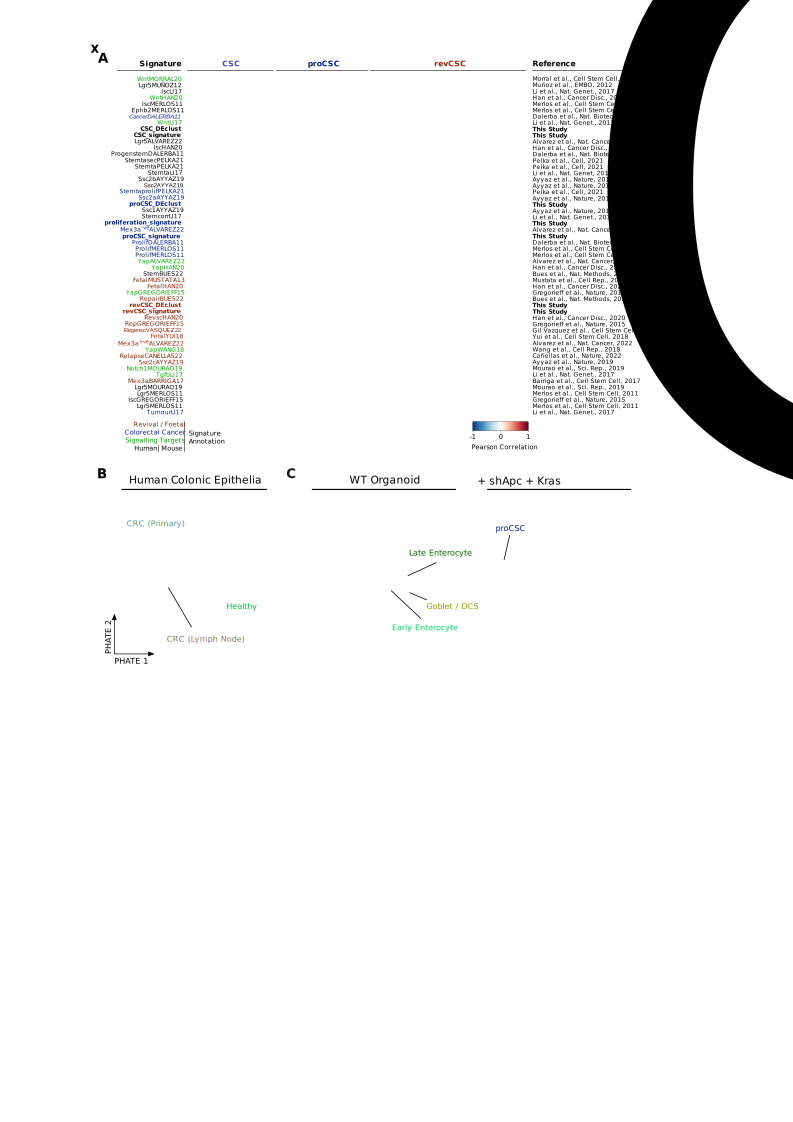
\includegraphics{04seq/figs/4SEQ_StemSign.png}
    \caption{\textbf{Epithelial Stem Cell Signatures.} \textbf{A)} Comparison of gene signatures of CSC, proCSC, and revCSC identified in this study with published stem cell signatures. \textbf{A)} CRC data comp.}
    \label{fig:4sign}
\end{figure}

As described in Chapter \ref{02methods}, literature signatures for diverse epithelial stem states and transcriptions targets of key signalling pathways were gathered (see \ref{tab:SignMD}) and projected on our data using UCell \cite{andreatta_ucell_2021}. The correlation of these signatures with our own reveals how the fibroblast-induced revCSC are indeed transcriptionally similar to "foetal" \cite{mustata_identification_2013, yui_yaptaz-dependent_2018} and "revival" stem cells \cite{ayyaz_single-cell_2019} of the intestinal epithelia at large (\ref{fig:4sign}A). 

The previously described association between revCSC and Yap and TGF-\textbeta\hspace{0.1cm}was also recovered by signature correlation, further validating the identity of the revCSC cluster. This observation, together with the cell-cell communication results, provided with the initial targets to pursue the mechanistic discovery of master regulators of the different stem states \cite{cardoso_rodriguez_single-cell_2023}.

In addition, proCSCs are transcriptionally comparable to stem cells observed in mouse and human CRC (Figure \ref{fig:4sign}A), showing a clear link with actively proliferating stem cell populations. CSC gene signatures are less common in CRC (Figure \ref{fig:4sign}A) and more closely resemble general pan-stem states.

This link between our mouse organoids and CRC patient data was further explored by comparing the murine organoids with aggregated data from several CRC cohorts in Joanito \emph{et al.}~\cite{joanito_single-cell_2022}. This resource contains both tumour and normal tissue samples that could be resolved on an integrated space of their scRNA-seq profiles (Figure \ref{fig:4sign}B). After cross species integration and projection of the mouse organoid data, one can non-quantitatively observe how the WT organoid cells align with normal tissue, whereas AK organoids align with cancer samples (Figure \ref{fig:4sign}C). 
%Also correlation between our proCSC and revCSC signatures was observed with the studies iCMS3 and iCMS2 respectively (Figure \ref{fig:4sign}D).

\newpage
\section{Conclusions}

% \colorbox{yellow}{OUTLINE (WIP)}
% * scRNA-seq dissect complex hetero organoid setting. 
% * Heterogeneous stem compartment.
% * proliferative stem cells and revival stem cells.
% * proCSC regulated by intrinsic oncogenic cues, revCSC by stromal signals.
% * WENR ligands regulate both, suggesting shared landscape of regulation orchestrated by wnt and egf.
% * intrinsic oncogenic cues compete, and win, against extrinsic cues however. At least part due to receptor downregulation in cancer organoids.
% * These populations and thus organoid as a whole, seem to have previously been found in the literature. Substantiate findings and model used.

In this chapter I have shown how \acrshort{scrnaseq} can be used to dissect the complex heterocellular setting of the organoid platform used. I have provided with an in-depth description of colonic epithelial differentiation and polarisation of its stem compartment. Furthermore, \emph{in silico} predictions regarding the mechanisms regulating these processes can also be formulated, which can (and have been in Qin \& Cardoso Rodriguez \emph{et al.}~\cite{cardoso_rodriguez_single-cell_2023}) be functionally validated using alternative single-cell \emph{omic} approaches (\acrshort{mc}).

On the unperturbed control, the WT organoid monocultures recapitulate the axis of differentiation from stem and basal states towards secretory and absorptive compartments. However I was unable to discern between discrete states within the secretory populations, with data from similar murine small intestinal organoids revealing the same observation, suggesting a putative limitation of the organoid model when compared to the \emph{in vivo} setting.

The finding of a heterogeneous stem compartment that can be so drastically polarised by stromal and oncogenic perturbations immediately stands out as the central observation of this study, revealing that fibroblasts and oncogenic mutations induce distinct epithelial stem cell-fates in colonic epithelia. I found that fibroblasts, potentially through the secretion of signalling ligands linked with WNT and TGF-\textbeta1, polarise epithelia towards slow-cycling CLU\textsuperscript{+} \acrshort{revcsc}s. In contrast, simultaneous APC-loss and oncogenic KRAS\textsuperscript{G12D} collaboratively block cell-extrinsic regulation of epithelial plasticity by interrupting stromal-epithelial communication, and polarise the organoids towards the hyper-proliferative \acrshort{procsc} state. By comparing the transcriptomic profiles of the stem states with the literature, I was able to validate both their identity and the link between \acrshort{revcsc} and TGF-\textbeta1 and YAP signalling, while also validate the organoid model as a whole.

The addition of WENR-enriched media revealed that exogenous WNT and EGF ligands can polarise the epithelium towards all stem states, at the expense of the differentiated cell states. The paired analysis on Qin \& Cardoso Rodriguez \emph{et al.}~\cite{cardoso_rodriguez_single-cell_2023} shows how CRC organoids can still access revival stem cells, but this requires high cell-extrinsic activation of YAP via TGF-\textbeta1 in parallel with reduced PI3K signalling. 

The CCAT pluripotency metrics and RNA velocity results are orthogonal methods that both paint a shared picture of competing transition and differentiation in which \acrshort{procsc} gives rise to differentiated states in the unperturbed organoids, but can be polarised towards alternatives fates like \acrshort{revcsc} (via extrinsic cues) or trapped in the \acrshort{procsc} state by oncogenic mutations.

These results demonstrate that colonic epithelia exist on a continuous differentiation landscape where oncogenic mutations and stromal cues compete for epithelial identity. However it appears that the former eventually dominate the extrinsic cues by blocking the stromal regulation of cell-fate plasticity. 
